%!TEX root = ../3dbook.tex

\setchapterpreamble[u]{\margintoc}

\graphicspath{{brep/}}
% \renewcommand*{\thelesson}{1.2}

\chapter{Boundary representation}%
\label{chap:brep}

In the first chapter, we discussed how 3D modelling is done through a series of abstractions of the real world.
One of the chief reasons to do so is to decrease the complexity of what needs to be modelled at each step, with the aim to successively break complex problems into simpler problems until they can be (more easily) solved.

\emph{Boundary representation} works using this principle.
Rather than modelling a 3D object through a volumetric representation, it instead models the object \emph{implicitly} by representing the 2D surface that bounds it (Figure~\ref{fig:cube}).
In this way, it is possible to use one of the many data structures that are used to represent 2D meshes, which are significantly simpler than the data structures used to directly represent arbitrary volumes.

\begin{marginfigure}
\centering
\includegraphics[width=\linewidth]{figs/cube.pdf}
\caption[A cube represented implicitly based on the six square faces that bound it]{A cube can be represented implicitly based on the six square faces that bound it.}%
\label{fig:cube}
\end{marginfigure}

However, it is very important to note that not all 3D objects can be represented using boundary representation with most common 2D mesh data structures without issues.
The main culprits are \emph{non-manifold} objects, which have properties that make representing them ambiguous, as well as objects with holes, which need to be stored using certain techniques.
External data structures might also be needed to keep track of disconnected set of objects, since it might not be possible to have access to them otherwise.

\section{What is boundary representation?}

Boundary representation\marginnote{boundary representation}\index{boundary representation}, also known as \emph{b-rep}\marginnote{b-rep}\index{b-rep} or \emph{surface modelling}\marginnote{surface modelling}\index{surface modelling}, is a method that involves representing an \(n\)-dimensional object through its \((n-1)\)-dimensional boundary.
Most of the time this term is used in the context of 3D modelling, where the aim is to represent a 3D object implicitly through its 2D boundary.
That being said, boundary representation is also common in 2D as well, where we sometimes represent polygons based on the line segments that bound them, and it is the main method used in 1D, where most of the time we represent line segments based on the two points that bound them (Figure~\ref{subfig:line})---as opposed to representing them based on something like a line equation.
Boundary representation can thus be used several times when representing a single 3D model: to represent a 3D volume as a set of 2D surfaces, each 2D surface as a set of 1D line segments or curves, and each 1D line segment as a pair of 0D points---or often 2D polygonal surfaces directly as sequences of 0D points (Figure~\ref{subfig:loop}).

\begin{figure}
\centering
\begin{subfigure}[b]{0.2\linewidth}
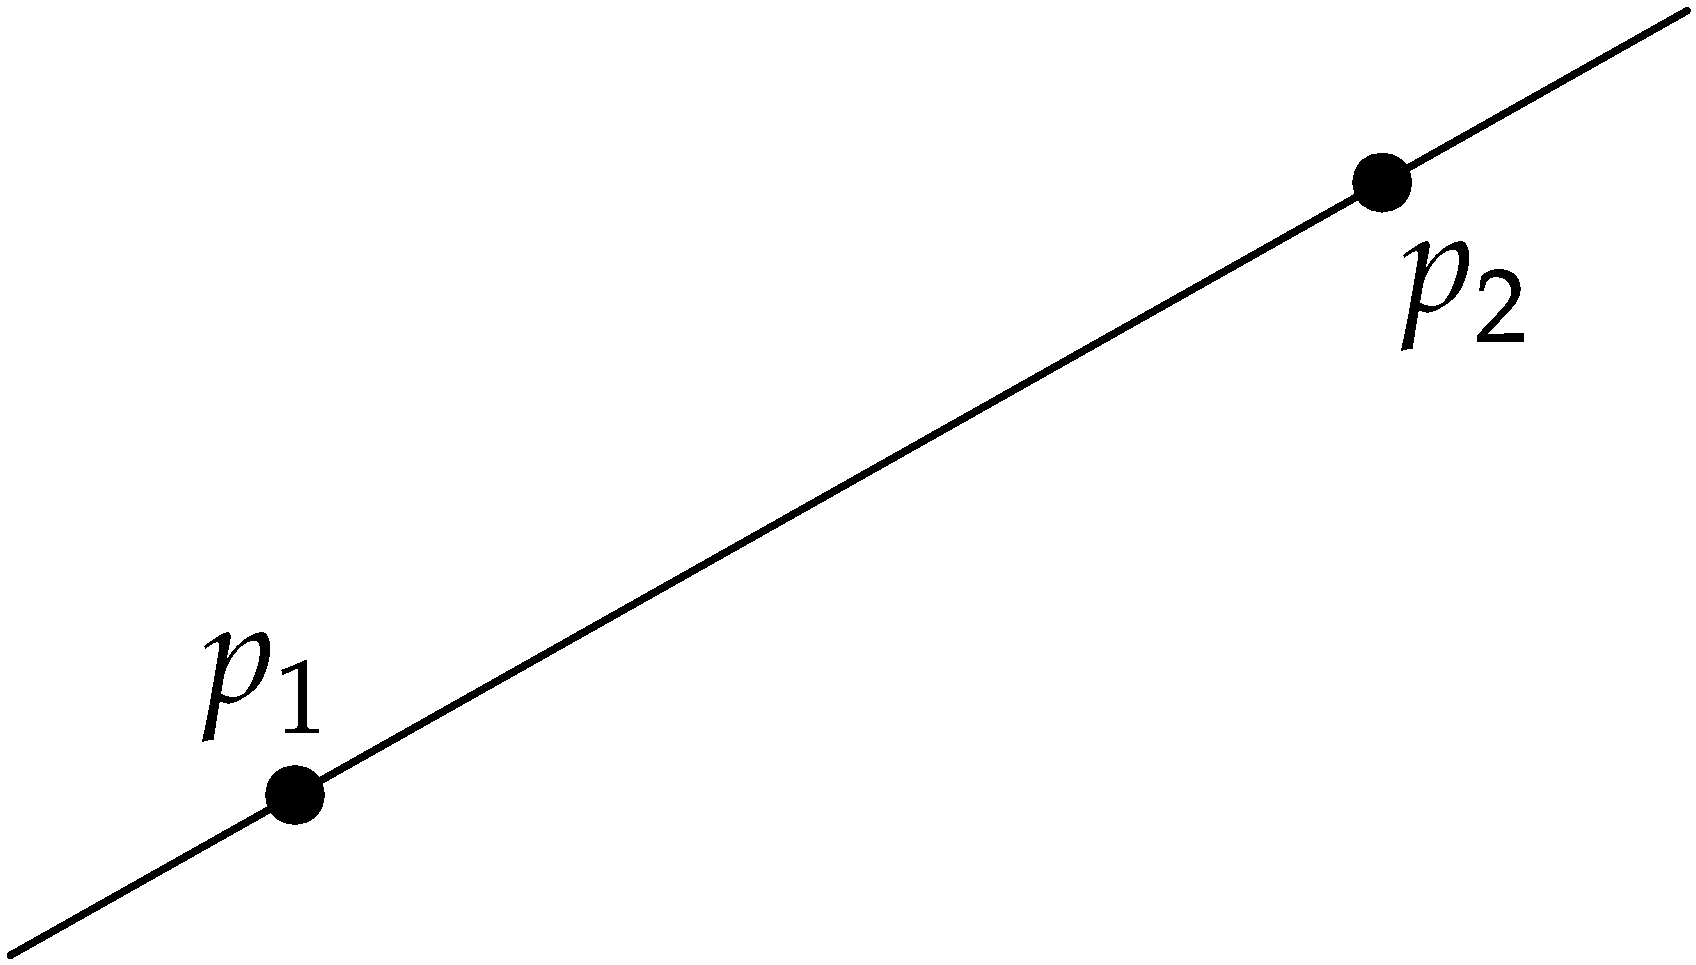
\includegraphics[width=\linewidth]{figs/line.pdf}
\caption{}%
\label{subfig:line}
\end{subfigure}
\quad
\begin{subfigure}[b]{0.3\linewidth}
\includegraphics[width=\linewidth]{figs/loop.pdf}
\caption{}%
\label{subfig:loop}
\end{subfigure}
\caption[Boundary representation]{Boundary representation as applied to: (a) 1D line segments represented implicitly through their two bounding points, and (b) a polygon represented by implying that it is bounded by a set of line segments, which are themselves bounded by consecutive pairs of points in a sequence of points (plus the last and the first).}%
\label{fig:brep}
\end{figure}

Boundary representation works because of what is known in 2D as the Jordan curve theorem\marginnote{Jordan curve theorem}\index{Jordan curve theorem}, which states that a closed curve separates the plane into two parts: an \emph{interior} surface and an \emph{exterior} surface.
In practical terms, this means that if you draw a closed curve (\ie\ a loop) on a sheet of paper, the curve separates the sheet into two parts---an interior one that is bounded on the outside by the curve, and an exterior one that is bounded on the outside by the edges of the sheet (\ie\ its outer boundary) and on the inside by the curve (\ie\ as an inner boundary).
In higher dimensions, this principle is known as the Jordan-Brouwer theorem\marginnote{Jordan-Brouwer theorem}\index{Jordan-Brouwer theorem}, which in 3D says that a closed surface separates 3D space into two parts: an interior volume and an exterior volume.

For our purposes, what the above theorems mean is that if we have a comprehensive method to represent a 2D surface, we can also use it to implicitly represent many 3D volumes with minimal modifications.
The specifics of these modifications depend on the data structure that we are using, but it often is as simple as adding an extra coordinate for each point (\ie\ $(x, y)$ becoming $(x, y, z)$).

\section{Objects with holes}

As hinted in the last paragraph, there are however some 3D volumes that are tricky to store using boundary representation.
The most obvious ones are \emph{objects with 3D holes} (\ie\ cavities)\marginnote{hole}\index{hole}\marginnote{cavity}\index{cavity}, since just like the paper sheet example described previously, they are bounded by one outer surface and possibly several inner surfaces (one per cavity).
Less obviously, objects with 2D faces with holes can have exactly the same problem with certain data structures (Figure~\ref{subfig:hole}), since a surface can be bounded by an outer ring and possibly multiple inner rings.

\begin{figure}
\centering
\begin{subfigure}[b]{0.3\linewidth}
\includegraphics[width=\linewidth]{figs/hole}
\caption{}%
\label{subfig:hole}
\end{subfigure}
\quad
\begin{subfigure}[b]{0.3\linewidth}
\includegraphics[width=\linewidth]{figs/hole-split}
\caption{}%
\label{subfig:hole-split}
\end{subfigure}
\begin{subfigure}[b]{0.3\linewidth}
\includegraphics[width=\linewidth]{figs/hole-bridge}
\caption{}%
\label{subfig:hole-bridge}
\end{subfigure}
\caption[Two different techniques to handle holes]{Two different techniques to handle holes in (a) a volume with 2D faces with holes: (b) splitting the volume into two parts and (c) using a bridge edge.}%
\label{fig:hole}
\end{figure}

Both of these cases are problematic for the same reasons.
In the simplest case, it can be because of a data structure is only built to store one ring/surface (\eg\ a single list of vertices for a ring).
However, the most common issue is that even when multiple rings/surfaces can be stored, the structures representing holes can end up separated from the rest of the data structure, resulting in a \emph{disconnected graph}\marginnote{disconnected graph}\index{disconnected graph}.
In other words, it might be impossible to navigate from the outer boundary of an object to its inner boundaries and vice versa.

While holes can cause problems when modelling objects using boundary representation, these are relatively easy to solve.
The three most common approaches are: 
\begin{enumerate}
	\item splitting volumes into multiple parts in such a manner that the 2D or 3D holes lie between different objects (Figure~\ref{subfig:hole-split}), then somehow semantically marking that the parts belong to the same object (\eg\ by using the same attribute id); 
	\item storing holes just like other (filled) objects, marking them as holes semantically (\eg\ with a special attribute or id), and then storing a list of holes for each object as a sort of attribute, from which they can then be easily accessed;
	\item using one \emph{bridge edge}\marginnote{bridge edge}\index{bridge edge} per hole, which are special edges that join each inner boundary to the outer boundary (Figure~\ref{subfig:hole-bridge}).
	The end result of this approach is that objects are only bounded by a single outer boundary, which wraps around the original outer boundary and all of the former inner boundaries.
	Bridge edges might also be marked semantically as such, although it is possible to tell that an edge is a bridge edge because it is surrounded on all sides by the same 2D/3D object.
\end{enumerate}

% A very similar case to objects with holes are disconnected (\ie\ non-touching) objects, which also result in a disconnected graph.
% In order to support these objects, many data structures have an explicit list of all existing objects, from which it is possible to access them.
% This list can be as simple as an array of pointers or ids, or as complex as a spatial index (\eg\ an R-Tree or $k$-d tree).

\section{Non-manifolds}

In addition to the above mentioned objects with holes, the other kind of objects that are tricky to store using boundary representation are \emph{non-manifolds}\marginnote{non-manifold}\index{non-manifold}.
However, in order to precisely describe what these are, we need to introduce some concepts from topology, which will allow us to describe them in terms of topological characteristics.

Mathematically, a \emph{homeomorphism}\marginnote{homeomorphism}\index{homeomorphism} is a continuous function that also has a continuous inverse.
This is a sort of equivalence relation (\(=\)) in topology, and so it can be used to tell that two objects are topologically equivalent or \emph{homeomorphic}.
In informal terms, applying a homeomorphism is like continuously deforming an object (without making holes in it or glueing different parts of it).
If an object can be transformed to another through this process, they are said to be homeomorphic (Figure~\ref{fig:homeomorphism}).
Homeomorphisms are important because of one key characteristic: they preserve all topological properties.
This means that they can be used to relate an arbitrary object to a simpler well-known one, which then has known topological properties (\eg\ Euclidean 2D space or a sphere).

\begin{figure}[htbp]
\centering
\begin{subfigure}[b]{0.4\linewidth}
\includegraphics[width=\linewidth]{figs/mug}
\caption{}%
\label{subfig:mug}
\end{subfigure}
\quad
\begin{subfigure}[b]{0.4\linewidth}
\includegraphics[width=\linewidth]{figs/donut}
\caption{}%
\label{subfig:donut}
\end{subfigure}
\caption[A typical joke about topology]{A typical joke about topology says that (a) a coffee mug and (b) a donut are homeomorphic.}%
\label{fig:homeomorphism}
\end{figure}

A \emph{manifold}\marginnote{manifold}\index{manifold} is a shape that is homeomorphic to the Euclidean space of a certain dimension, \ie\ a point in 0D, a line in 1D, a plane in 2D or 3D space in 3D.
An intuitive way to think about this is that a manifold locally resembles Euclidean space, even if globally it does not.
For example, a line and a circle are both 1-manifolds, while a plane, a sphere and a torus are all 2-manifolds.
Meanwhile, non-manifolds\marginnote{non-manifold}\index{non-manifold} are shapes where you can find at least one point where this condition is not true (Figure~\ref{subfig:nonmanifold-0} and~\ref{fig:non2manifold}).
In geomatics, when people refer to a non-manifold, they are usually referring to a non-2-manifold in the context of modelling a 3D object using boundary representation.

\begin{figure}
\centering
\begin{subfigure}[b]{0.3\linewidth}
\includegraphics[width=\linewidth]{figs/nonmanifold-0}
\caption{}%
\label{subfig:nonmanifold-0}
\end{subfigure}
\quad
\begin{subfigure}[b]{0.3\linewidth}
\includegraphics[width=\linewidth]{figs/nonmanifold-1}
\caption{}%
\label{subfig:nonmanifold-1}
\end{subfigure}
\quad
\begin{subfigure}[b]{0.3\linewidth}
\includegraphics[width=\linewidth]{figs/nonmanifold-2}
\caption{}%
\label{subfig:nonmanifold-2}
\end{subfigure}
\caption[A 1D boundary around a polygon that is non-1-manifold]{(a) The 1D boundary around a polygon is a non-1-manifold because the space around a vertex (highlighted in a red circle) is not homeomorphic to a line. (b) \& (c) However, the polygon can still be represented using a loop of oriented edges by creating a duplicate vertex at that location (shown as two half disks), but there are two ways in which this can be done.
Note that these are not equally desirable as (c) results in a disconnected structure (just like a hole).}%
\label{fig:nonmanifold}
\end{figure}

Based on these definitions, we can now better describe exactly which 3D objects can be stored using boundary representation without problems: those that are bounded by exactly one 2-manifold surface.
The intuitive logic that explains this is: 2D space is (by definition) a 2-manifold surface, which means that we are able to store objects that are bounded by a surface that is homeomorphic to it.
Another intuitive way to think about this is to consider a counterexample in terms of the Jordan curve theorem: if we draw a closed loop that crosses itself (\eg\ the number 8), which is clearly a non-manifold, we will end up with more than one interior part (or possibly an ambiguous situation).

\begin{marginfigure}
\centering
\includegraphics[width=\linewidth]{figs/non2manifold.jpg}
\caption[A 2D surface around a volume that is non-2-manifold]{The 2D surface around this volume is a non-2-manifold because it is not homeomorphic to a plane.}%
\label{fig:non2manifold}
\end{marginfigure}

While the obvious solution might be to disallow non-manifold objects, they are common in practice, and so we need to have methods to deal with them, even if these methods might introduce additional complexity to boundary representation.
In order to overcome this problem, there are two approaches that are typically used:

\begin{enumerate}
	\item splitting non-manifold objects into multiple manifold parts, then marking the parts as belonging to the same object using semantics;
	\item creating duplicate elements at the same location (Figure~\ref{subfig:nonmanifold-1} and~\ref{subfig:nonmanifold-2}).
		In 2D this usually involves duplicate vertices, whereas in 3D this might involve duplicate edges as well.
\end{enumerate}

\section{Topological concepts}

In addition to holes and manifolds, there are other topological concepts that are commonly used when characterising objects in 3D modelling.
These are not directly related to the present chapter, but we will make a small tangent to introduce them here.

The \emph{genus}\marginnote{genus}\index{genus} of a surface is the maximum number of closed loop cuts we can make in it without causing it to become disconnected (Figure~\ref{fig:genus}).
Note the `maximum' here, since it is always possible to select loops that cause a surface to become disconnected.
Intuitively, it is the number of `handles' it has.
A sphere thus has genus 0, whereas a torus (\eg\ the donut and coffee mug) have genus 1 because we can cut the handle of the object and still have a connected surface.

\begin{figure}
\centering
\begin{subfigure}[b]{0.3\linewidth}
\includegraphics[width=\linewidth]{figs/genus1}
\caption{}%
\label{subfig:genus1}
\end{subfigure}
\quad
\begin{subfigure}[b]{0.3\linewidth}
\includegraphics[width=\linewidth]{figs/genus2}
\caption{}%
\label{subfig:genus2}
\end{subfigure}
\quad
\begin{subfigure}[b]{0.3\linewidth}
\includegraphics[width=\linewidth]{figs/genus3}
\caption{}%
\label{subfig:genus3}
\end{subfigure}
\caption[Surfaces with different genus]{Surfaces with: (a) genus 1, (b) genus 2, (c) genus 3. From Wikimedia Commons.}%
\label{fig:genus}
\end{figure}

A surface is said to be \emph{orientable}\marginnote{orientability}\index{orientability} when it is possible to define a normal vector at every point of the surface in a consistent manner, \ie\ without sudden reversals of the vector direction when moving long the surface.
Since real-world objects are always orientable (Figure~\ref{fig:mobius}), this might seem like a non-issue in practice.
However, real-world objects are always volumetric---no matter how thin they are---but when these are modelled, they are often modelled as surfaces (\ie\ without thickness), which makes it possible to have unorientable surfaces.

\begin{figure}
\centering
\includegraphics[width=0.6\linewidth]{figs/mobius}
\caption[A M\"obius strip]{A M\"obius strip is a one-sided surface, equivalent to glueing a paper strip with a single 180\(^\circ\) twist, and it is the most typical example of a non-orientable surface. Note however that this is only true when it is modelled without thickness. From Wikimedia Commons.}%
\label{fig:mobius}
\end{figure}

\section{Data structures for meshes}

Moving back to the storage of 3D models using boundary representation, there are a large number of data structures that can be used for this purpose.
However, there are three broad approaches: (i) data structures using triangles as base elements; (ii) data structures that use edges or half-edges as base elements; and (iii) data structures that have polygons, edges and vertices as base elements.
We will show one or two characteristic examples for each approach, with the understanding that there are many possible variations of each of them.

\subsection{Triangle-based structures}

The first typical approach relies on a surface being triangulated, \ie\ being split entirely into triangles, so that you have a triangle mesh\marginnote{triangle mesh}\index{triangle mesh}.
This is often desirable because in a triangle mesh, each triangle is known to have only up to three adjacent triangles and only up to three incident vertices, whereas in a polygon it can be any number.
Because of this, a triangle-based data structures (Figure~\ref{fig:2-simplex}) can use fixed-length data structures to store all their elements (\eg\ arrays), which are more efficient.

\begin{figure}
\centering
\begin{subfigure}[b]{0.27\linewidth}
\includegraphics[width=\linewidth]{figs/2-simplex-adjacency}
\caption{}%
\label{subfig:2-simplex-adjacency}
\end{subfigure}
\quad
\begin{subfigure}[b]{0.27\linewidth}
\includegraphics[width=\linewidth]{figs/2-simplex-vertices}
\caption{}%
\label{subfig:2-simplex-vertices}
\end{subfigure}
\quad
\begin{subfigure}[b]{0.27\linewidth}
\includegraphics[width=\linewidth]{figs/0-simplex}
\caption{}%
\label{subfig:0-simplex}
\end{subfigure}
\caption[A triangle-based data structure]{A triangle-based data structure consists of a set of triangles as base elements, each of which has links to (a) its three adjacent triangles (as pointers or ids).
Then, the usual approach is to also have links to (b) its three incident vertices (as pointers or ids), which can stored as separate elements with (c) their coordinates.
Alternatively, it is also possible to store the vertex coordinates directly in the triangles, but this means that the coordinates are stored many times---once in every triangle that is incident to it.}%
\label{fig:2-simplex}
\end{figure}

Since there are specific elements for triangles and vertices, triangle-based data structures make it easy to store attributes both for triangles and for vertices.
For instance, it is possible to mark all the triangles belonging to a certain surface semantically through the use of a common attribute, which could be a pointer or id linking to a surface element.
Such a surface could contain attributes common to all the triangles that represent it.

Surfaces with holes are generally not a problem for triangle-based data structures.
When these are triangulated (using a constrained triangulation), holes become connected to the rest of the structure.
If a hole of a surface contains a different surface, the triangles adjacent to it can simply link to the triangles representing it.
If it does not, the triangles can have a special link or value corresponding to empty space (\eg\ null).
The same applies for triangles on the edge of the surface

In addition to the basic approach, there are variations that use more compact representations of triangle-based structures, usually by joining multiple adjacent triangles that are arranged in a certain way.
Examples of these are triangle strips (Figure~\ref{fig:trianglestrip}) and triangle fans/stars (triangles that are all incident to a certain vertex).

\begin{marginfigure}
\centering
\includegraphics[width=\linewidth]{figs/trianglestrip}
\caption[A triangle strip is easily defined as a list of vertices]{A triangle strip is easily defined as a list of vertices \((a,b,c,d,e,f,g,h)\). Every triangle is formed by three consecutive vertices in the list.}%
\label{fig:trianglestrip}
\end{marginfigure}

\subsection{Edge-based structures}

When we want to allow for polygons in a surface, the most common approach is to use data structures where the base elements are either edges or half-edges.
Let us look at one example of each.

The \emph{quad-edge}\marginnote{quad-edge data structure}\index{quad-edge data structure} data structure uses edges as base elements.
Each edge then stores what is known as a \emph{quad}\marginnote{quad}\index{quad} (Figure~\ref{fig:quad}) and links to one or both of its incident vertices.
Note that these quads are named as such because they store four piece of information and are unrelated to quads (\ie\ quadrilaterals) in computer graphics.

In a common easy implementation of the quad-edge data structure, the edge is first given an arbitrary orientation.
In this manner, there are vertices at the \emph{start} and \emph{end} of the edge, which can be used as names to access them, and there are thus \emph{left} and \emph{right} polygons, which means that the quad links can thus be called something like \emph{left-previous}, \emph{left-next}, \emph{right-previous} and \emph{right-next}.

\begin{figure}[b]
\centering
\includegraphics[width=0.7\linewidth]{figs/quad}
\caption[In the quad-edge data structure, an edge stores a \emph{quad}]{In the quad-edge data structure, an edge stores a \emph{quad}, which contains four records pointing to other quads corresponding to the previous and next oriented edges for the polygons on both of its sides.}%
\label{fig:quad}
\end{figure}

While this approach works fine, it is important to note that there will not be a consistent orientation between adjacent edges.
That is, polygons will not be defined by an oriented loop of edges going around them.
Vertices can thus have multiple edges pointing away from them and toward them.
As an example of the consequences of this, getting all the vertices of a polygon is a bit awkward, since for each iteration where we arrive at an edge, we need to check the orientation of the edge and program a different logic for each orientation.

The alternative is to split each edge into two linked half-edges with opposite orientations.
This approach is called the \emph{half-edge data structure}\marginnote{half-edge data structure}\index{half-edge data structure}, of which are many variations in practice, such as the doubly connected edge list (DCEL)\marginnote{DCEL}\index{DCEL}.
In the DCEL (Figure~\ref{fig:halfedge}), half-edges\marginnote{half-edge}\index{half-edge} are the base element, but there are also elements for vertices and faces.
Vertices store their coordinates and a link to one face-edge starting from it, whereas faces store a link to a half-edge on its outer boundary.
If holes are present, faces also typically store one link to a half-edge on each of its inner boundaries.
Note however that since a face can have any number of holes, this means that a variable-length data structure (\eg\ a linked list) will need to be used.
Vertices, half-edges and faces can each also contain fields for attributes.
Storing attributes for edges will thus result in duplicate information (or additional edge objects that are linked to both half-edges).

\begin{figure}
\centering
\begin{subfigure}[b]{0.27\linewidth}
\includegraphics[width=\linewidth]{figs/halfedge-1}
\caption{}%
\label{subfig:halfedge-1}
\end{subfigure}
\quad
\begin{subfigure}[b]{0.27\linewidth}
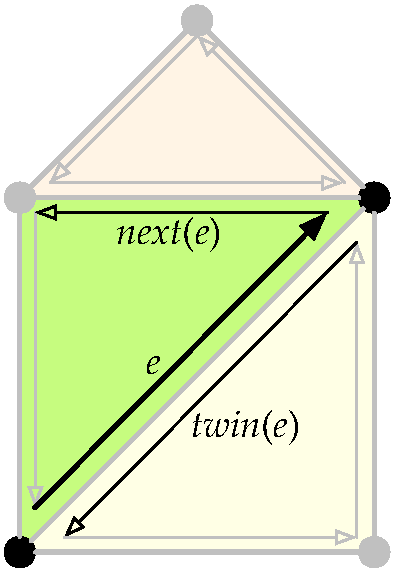
\includegraphics[width=\linewidth]{figs/halfedge-2}
\caption{}%
\label{subfig:halfedge-2}
\end{subfigure}
\caption[Three adjacent polygons are represented using the DCEL]{(a) Three adjacent polygons are represented using (b) the DCEL\@.
In the DCEL, a half-edge \(e\) is linked to two vertices (called the \emph{origin} and the \emph{destination}) and to the face that it is incident to, and is linked to its \emph{next} half-edge (on the same face) and its \emph{twin} half-edge (on the adjacent face).}%
\label{fig:halfedge}
\end{figure}

In general, half-edge data structures are more verbose than edge-based data structures.
However, they make navigating through the structure much easier.
For instance, obtaining all the vertices of a polygon in order in the DCEL simply involves finding a half-edge in the polygon, and then iteratively following the \emph{next} links until we get back to the original half-edge.

\subsection{Incidence graphs}

The last approach that is common in practice is the \emph{incidence graph}\marginnote{incidence graph}\index{incidence graph}.
It is a simple data structure where \(i\)-dimensional elements are linked to the \((i-1)\)-dimensional elements that bound it (Figure~\ref{fig:incidencegraph}).
This approach makes it easy to store attributes for faces, edges and vertices without redundancy.
However, it needs variable-length data structures to store the edges that bound each face.
Because of this, it is commonly used where this limitation is not a problem (\eg\ in text files), but it is avoided when efficiency is more important and where variable-length fields are a problem (\eg\ in databases).

\begin{figure}
\centering
\begin{subfigure}[b]{0.27\linewidth}
\includegraphics[width=\linewidth]{figs/2-cell-boundary}
\caption{}%
\label{subfig:2-cell-boundary}
\end{subfigure}
\quad
\begin{subfigure}[b]{0.27\linewidth}
\includegraphics[width=\linewidth]{figs/1-cell-boundary}
\caption{}%
\label{subfig:1-cell-boundary}
\end{subfigure}
\quad
\begin{subfigure}[b]{0.27\linewidth}
\includegraphics[width=\linewidth]{figs/0-cell-embedding}
\caption{}%
\label{subfig:0-cell-embedding}
\end{subfigure}
\caption[The incidence graph]{In the incidence graph, (a) faces have a list with links to the edges that bound them, (b) edges have links to the two vertices that bound them, and (c) vertices contain their coordinates.}%
\label{fig:incidencegraph}
\end{figure}

%%%
%
\section{Exercises}

\begin{enumerate}
	\item Why can we represent a 2D polygon directly as a sequence of 0D points (\ie\ skipping line segments entirely) but we cannot do the same in 3D\@?
	\item Exactly where is the surface of Figure~\ref{fig:non2manifold} not homeomorphic to a plane?
	\item Splitting objects is a simple solution to deal with both holes and non-manifolds. However, in terms of semantics it is often not desirable. Why is that?
	\item In a triangle fan or star, we need to store vertices in a specific order. Why is that?
	\item How can you obtain all the edges incident to a vertex in order (\ie\ as you rotate around the vertex) using the quad-edge data structure? How about for the DCEL\@? Which is easier?
\end{enumerate}



%%%
%
\section{Notes and comments}

The original place where the Jordan curve theorem is introduced is  \citet{Jordan87}, which is an old French textbook on calculus and differential equations.
The generalisation to higher dimensions was apparently done by \citet{Lebesgue11} and \citet{Brouwer11}, although this is somewhat contentious~\citep[Ch.~5]{van-Dalen13}.

% We mentioned R-trees and \(k\)-d trees as examples of spatial indices.
% The details of each are not very relevant here, but it is good to know that they have tree structures with links to each object in the leaves.
% If you want to get more familiar with them, you can skim the papers where they were introduced, \citet{Guttman84} and \citet{Bentley75}, or simply check the Wikipedia article for an R-tree: \url{https://en.wikipedia.org/wiki/R-tree}.

If you want to see how the coffee mug and the donut from Figure~\ref{fig:homeomorphism} are homeomorphic, watch this video: \url{https://www.youtube.com/watch?v=9NlqYr6-TpA}.

A nice description of a star-based data structure is available in \citet{Blandford05}, or in 3D in \citet{Ledoux13a}.

The quad-edge data structure was originally described in \citet{Guibas85}.
The first data structure of that type is likely the winged-edge data structure~\citet{Baumgart75}.

As for half-edge data structure, the first example is likely the 2D combinational map~\citep{Edmonds60}.
The DCEL is originally described in \citet{Muller78}, but you can find nicer descriptions in \citet{Worboys04} or \citet{deBerg08}.
